% 01_introduction.tex

Here is an example of a citation \cite{ref:oetiker1995not}. Citations are included in the \texttt{cited\_works.bib} file.

\blindtext

\subsection{Introduction Section \#1}
\label{sect:intro_1}

For an example of a figure with subfigures, see Fig~\ref{fig:ann_inputs} or~\ref{fig:ann_outputs}.

\blindtext 

\begin{figure}[htbp]
	\begin{subfigure}[t]{.45\textwidth}
		\centering
		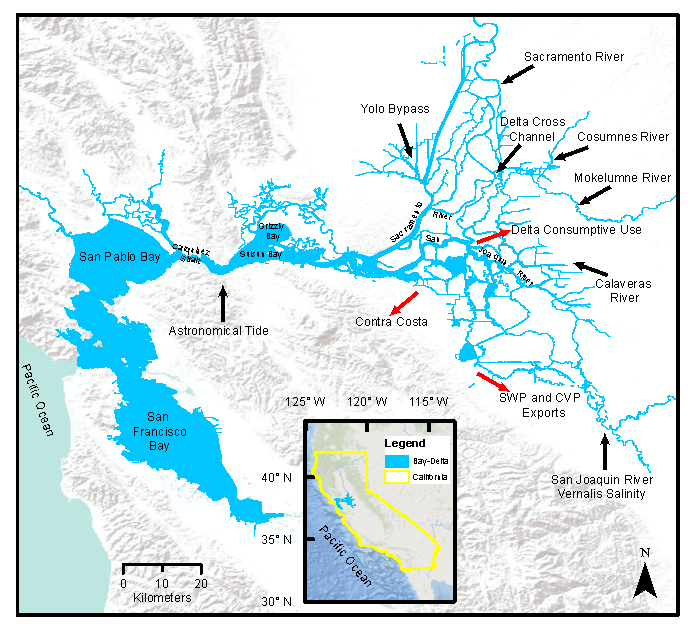
\includegraphics[width=\linewidth]{ann_inputs_he_Aug17.pdf}
		\caption{ANN inputs and input locations.}
		\label{fig:ann_inputs}
	\end{subfigure}
	\begin{subfigure}[t]{.45\textwidth}
		\centering
		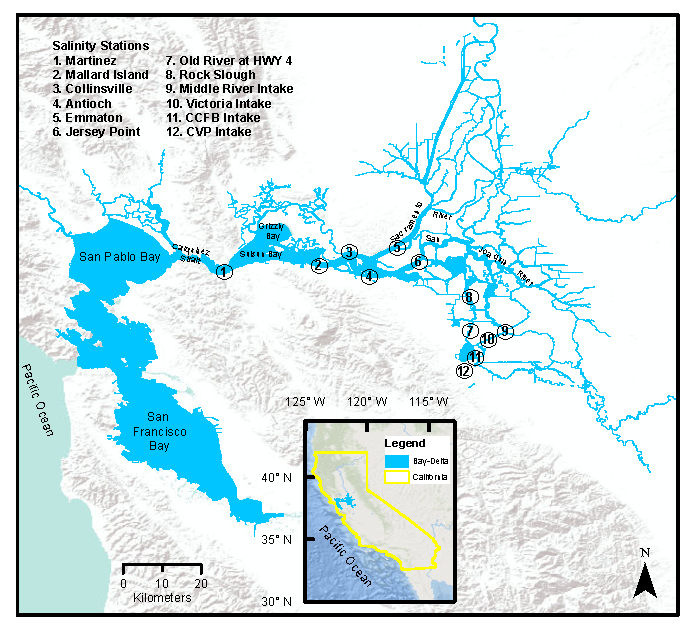
\includegraphics[width=\linewidth]{ann_outputs_he_Aug17.pdf}
		\caption{Locations of the 12 Study Salinity Stations.}
		\label{fig:ann_outputs}
	\end{subfigure}
\caption{ANN input and output locations in San Francisco Bay and Sacramento-San Joaquin Delta Estuary (Bay-Delta Estuary).}
\end{figure}

\subsubsection{MIMO Channel Overview}
\label{sect:mimo_model}

In this work, we consider a MIMO channel with a multiple antennas ($n_B \gg 1$) at the transmitter (gNodeB or gNB) servicing one or more user equipment (UE) with single antennas. The network utilizes orthogonal frequency division multiplexing (OFDM) with $N_f$ subcarriers, the $m$-th downlink and uplink channels at the receiver are given as
\begin{align*}
	y_{d,m} &= \mathbf h_{d,m}^H\mathbf w_{t,m}x_{d,m} + n_{d,m}, \\
	y_{u,m} &= \mathbf w_{r,m}^H\mathbf h_{u,m}x_{u,m} + \mathbf w_{r,m}^H\mathbf n_{u,m}.
\end{align*}
The resulting downlink and uplink CSI matrices are given as
\begin{align*} 
\overline{\mathbf H}_d &= \begin{bmatrix} \mathbf h_{d,1} & \dots & \mathbf h_{d,N_f}\end{bmatrix}^H \in \mathbb C^{N_f \times N_b}, \\
\overline{\mathbf H}_u &= \begin{bmatrix} \mathbf h_{u,1} & \dots & \mathbf h_{u,N_f}\end{bmatrix}^H \in \mathbb C^{N_f \times N_b}.
\end{align*}
\begin{table}[]
\centering
\caption{MIMO system parameters and variables considered in this work.}
\label{tab:cost-params}
\begin{tabular}{c|c|l}
\toprule
\textbf{Symbol}   & \textbf{Dimension}          & \textbf{Description} \\ \midrule
$y_{d,m}$ 		  & $\mathbb{C}^{1}$ 			& Received downlink symbol on $m$-th subcarrier  \\ \hline
$\mathbf h_{d,m}$ & $\mathbb{C}^{N_b \times 1}$ & Downlink impulse response on $m$-th subcarrier  \\ \hline
$\mathbf w_{t,m}$ & $\mathbb{C}^{N_b \times 1}$ & Transmitter precoding vector for $m$-th subcarrier  \\ \hline
$x_{d,m}$ 		  & $\mathbb{C}^{1}$ 			& Trasmitted symbol on $m$-th subcarrier  \\ \hline
$n_{d,m}$ 		  & $\mathbb{C}^{1}$ 			& Downlink noise on $m$-th subcarrier  \\ \hline
$y_{u,m}$ 		  & $\mathbb{C}^{1}$ 			& Received uplink symbol on $m$-th subcarrier  \\ \hline
$\mathbf h_{u,m}$ & $\mathbb{C}^{N_b \times 1}$ & Uplink impulse response on $m$-th subcarrier  \\ \hline
$\mathbf w_{r,m}$ & $\mathbb{C}^{N_b \times 1}$ & Received precoding vector for $m$-th subcarrier  \\ \hline
$x_{u,m}$ 		  & $\mathbb{C}^{1}$ 			& Received symbol on $m$-th subcarrier  \\ \hline
$\mathbf n_{u,m}$ & $\mathbb{C}^{1}$ 			& Uplink noise on $m$-th subcarrier  \\ \hline
\end{tabular}
\end{table}

\subsection{Introduction Section \#2}
\label{sect:intro_2}

\blindtext 

\subsection{Channel Model}
\label{sect:channel_model}

For all CSI tests, we mainly rely on the COST2100 MIMO channel model \cite{ref:liu2012cost2100}. We use two datasets with a single base station (gNB) and a single user equipment (UE) in the following scenarios:
\begin{enumerate}
	\item \textbf{Indoor} channels using a 5.3GHz downlink at
	0.001 m/s UE velocity, served by a
	gNB at center of a $20$m$\times 20$m coverage area.
	\item \textbf{Outdoor} channels using a 300MHz downlink at 0.9 m/s UE velocity served by a gNB at center 
	of a $400$m$\times 400$m coverage area.
\end{enumerate}
In both scenarios, we use the parameters listed in Table~\ref{tab:cost-params}.
\begin{table}[]
\centering
\caption{Parameters used for COST2100 simulations for both Indoor and Outdoor datasets.}
\label{tab:cost-params}
\begin{tabular}{c|c|l}
\toprule
\textbf{Symbol} & \textbf{Value} & \textbf{Description} \\ \midrule
$N_b$ 			& 32			 & Number of antennas at gNB  \\ \hline
$N_f$ 			& 1024			 & Number of subcarriers for OFDM link  \\ \hline
$R_d$ 			& 32			 & Number of delay elements kept after truncation  \\ \hline
$N$ 			& $10^6$		 & Total number of samples per dataset  \\ \hline
$T$ 			& 10		 	 & Number of timeslots  \\ \hline
$\delta$		& 40ms, 80ms	 & Feedback delay interval between consecutive CSI timeslots  \\ \bottomrule
\end{tabular}
\end{table}
